\documentclass{article}
\usepackage[utf8]{inputenc}
\usepackage[margin=0.8in]{geometry}

\title{Union-Find}
\author{Kevin Geng}
\date{30 September 2016}

\usepackage{graphicx}

\usepackage{algorithm}
\usepackage{algorithmicx}
\usepackage[noend]{algpseudocode}

\usepackage{tikz}
\usetikzlibrary{calc,shapes.multipart,chains,arrows,positioning}

\tikzstyle{vertex}=[draw,fill=myseagreen,circle,minimum size=24pt,inner sep=0pt]

\tikzstyle{splitvertex}=[draw,fill=myseagreen,circle split,minimum size=24pt]


% for black and white printing; see below
%\definecolor{myseagreen}{RGB}{88,197,191}
%\definecolor{mysalmon}{RGB}{255,160,122}
%\definecolor{myred}{RGB}{255,102,102}
%\definecolor{mypurple}{RGB}{225,145,255}

\definecolor{myseagreen}{RGB}{238,238,238}
\definecolor{mysalmon}{RGB}{204,204,204}
\definecolor{mypurple}{RGB}{170,170,170}

\definecolor{myblack}{RGB}{0,0,0}
\definecolor{mywhite}{RGB}{255,255,255}


\begin{document}

\maketitle

\section{Connectivity}

\subsection{Connected components}

To start our discussion, let's consider the idea of connected components. In an undirected graph\footnote{We will consider connectivity in directed graphs later this year.}, we say that two vertices are \textit{connected} if you can reach one from the other by traversing a series of edges. Then, a connected component is a subgraph such that any two vertices in the component are connected.

\begin{figure}[h]
\centering
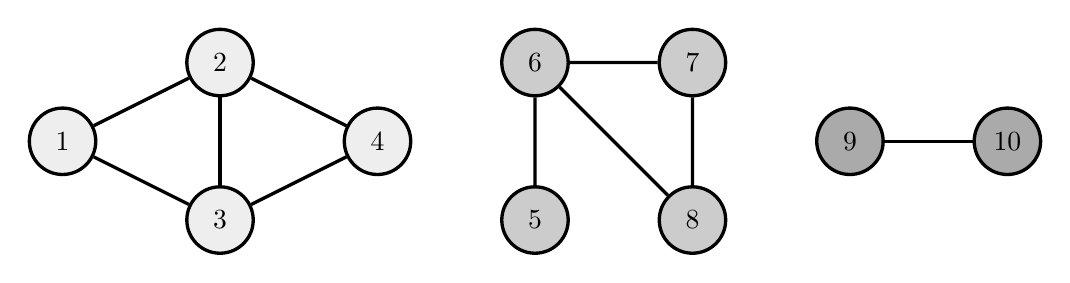
\begin{tikzpicture}[very thick,level/.style={sibling distance=70mm/#1}]
\draw (0, 0) node [vertex] (n1) {1};
\draw (2, 1) node [vertex] (n2) {2};
\draw (2, -1) node  [vertex] (n3) {3};
\draw (4, 0) node [vertex] (n4) {4};
\draw (n1) -- (n2);
\draw (n2) -- (n3);
\draw (n3) -- (n4);
\draw (n2) -- (n4);
\draw (n1) -- (n3);
\draw (6, -1) node [vertex, fill=mysalmon] (n5) {5};
\draw (6, 1) node [vertex, fill=mysalmon] (n6) {6};
\draw (8, 1) node [vertex, fill=mysalmon] (n7) {7};
\draw (8, -1) node [vertex, fill=mysalmon] (n8) {8};
\draw (n5) -- (n6) -- (n7) -- (n8) -- (n6);
\draw (10, 0) node[vertex, fill=mypurple] (n9) {9};
\draw (12, 0) node[vertex, fill=mypurple] (n10) {10};
\draw (n9) -- (n10);
\end{tikzpicture}
\caption{This diagram illustrates a graph with three connected components. \textit{Credit: Samuel Hsiang}}
\end{figure}

To determine the connected components in a graph, we can simply perform a flood-fill on the graph. Specifically, for each of the vertices in the graph, we can determine what other vertices are connected to it using DFS or BFS, then mark them as belonging to the same component with an identifier unique to the component. This runs in $O(V+E)$ time.


\subsection{Dynamic connectivity}
The \textit{dynamic connectivity} problem is an extension of the problem of connectivity. We want to be able to add edges to a graph, but also determine the connected components of that graph at any time. However, for the purposes of this lecture, we will not consider removing edges.

Alternatively, we can consider the problem in terms of two operations that we would like to perform on an undirected graph:

\begin{itemize}
    \item \textit{find(p):} Determine which connected component a vertex $p$ is in. Note that we can easily determine whether two vertices are connected by checking whether they are in the same connected component.
    \item \textit{union(p, q):} Connect two vertices $p$ and $q$ in the graph.
\end{itemize}

We can also think of this problem in terms of elements in subsets, instead of vertices in components. Though we need to know what vertices in a connected component, we do not need to know how those vertices are connected, because they are all connected to each other.\footnote{This is because connectivity is an \textit{equivalence relationship}: it is reflexive, symmetric, and transitive.} This frees us from the constraints of the data structures that we use for graphs, such as adjacency lists.


\pagebreak

\section{Union-find (Disjoint-set)}

The goal of the \textit{union-find data structure}, or the \textit{disjoint-set data structure} is to efficiently solve the dynamic connectivity problem. Instead of using a graph representation, for each node, we can maintain a parent pointer to one other node that it's connected to. Eventually, following these pointers will lead to a root node that does not point to anything. Since all nodes in the component point to it, it is the \textit{representative element} of the component. This forms a collection of trees, also known as a \textit{forest}.

\begin{figure}[h]
\centering
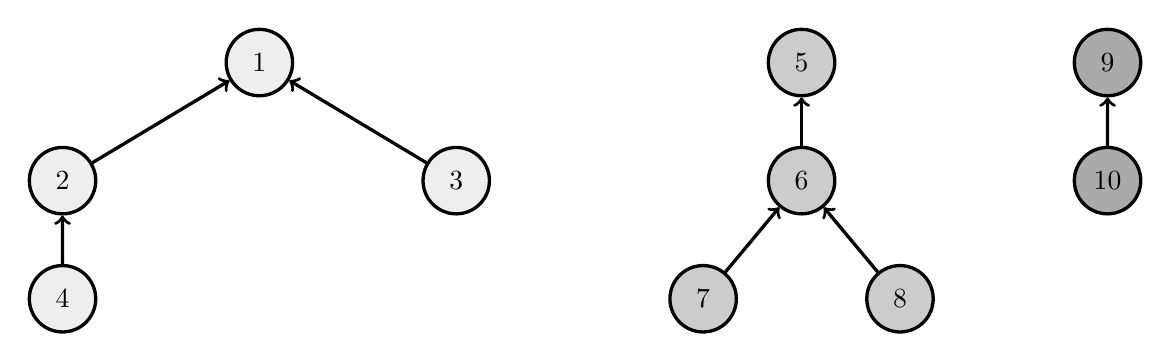
\begin{tikzpicture}[very thick,edge from parent/.style={draw,<-},level/.style={sibling distance=50mm/#1}]
\node [vertex, fill = mysalmon] (r2) {5}
  child {
      node [vertex, fill = mysalmon] {6}
      child { node [vertex, fill=mysalmon] {7} }
      child { node [vertex, fill=mysalmon] {8} }
  };

\node [vertex] [left=6cm of r2] (r1) {1}
  child {
    node [vertex] {2}
    child {
      node [vertex] {4}
    }
  }
  child {node [vertex] {3} };
  
\node [vertex, fill=mypurple] [right=3cm of r2] (r3) {9}
  child { node [vertex, fill=mypurple] {10} };
\end{tikzpicture}
\caption{Representation of union-find as a forest. \textit{Credit: Samuel Hsiang}}
\end{figure}

If we number our nodes sequentially, we can easily represent these pointers in an array instead. Instead of a null parent pointer, root nodes will point to themselves.

\begin{figure}[h]
\centering
{
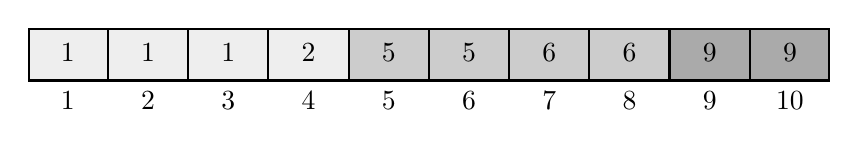
\begin{tikzpicture}[
  thick,
  myrect/.style={
    draw,
    rectangle split,
    rectangle split horizontal,
    rectangle split parts=#1,
    rectangle split part align=left,
    text width=5ex,
    text centered
    },
  mycallout/.style={
    shape=rectangle callout,
    rounded corners,
    fill=mysalmon,
    callout absolute pointer={#1},
    callout pointer width=1cm
  }  
]

\node[myrect=10, rectangle split part fill={myseagreen, myseagreen, myseagreen, myseagreen, mysalmon, mysalmon, mysalmon, mysalmon, mypurple, mypurple}]
  (array1)
  {
  					\strut 1
  \nodepart{two}	\strut 1
  \nodepart{three}	\strut 1
  \nodepart{four}	\strut 2
  \nodepart{five}	\strut 5
  \nodepart{six}	\strut 5
  \nodepart{seven}	\strut 6
  \nodepart{eight}	\strut 6
  \nodepart{nine}	\strut 9
  \nodepart{ten}	\strut 9
  };
\foreach \Valor [count=\Valori from 1] in {one ,two ,three ,four ,five ,six ,seven ,eight ,nine ,ten }
  \node[below] at (array1.\Valor south) {\Valori};

\end{tikzpicture}
}
\caption{Representation of union-find as an array. \textit{Credit: Samuel Hsiang}}
\end{figure}

\section{Quick-find}

One way to implement \textit{Union} and \textit{Find} is to have every node directly point to the root node of the component. In fact, this is the same data structure that we used to solve the connected components problem.

\begin{itemize}
    \item \textit{find(p):} Return the value at index $p$ of the array, the index of the connected component's root.
    \item \textit{union(p, q):} Search the array. For every element that contains the value $q$, replace it with $p$.
\end{itemize}

Now we have an algorithm that runs in $O(1)$ time for \textit{find()}, but $O(N)$ time for \textit{union()}. However, this is the same time complexity that we would get by simply performing a flood-fill every time we ran \textit{union()}. We can do better.


\section{Quick-union}

With quick-find, we update every element in one connected component whenever we perform a union, which requires us to search the entire array. Instead, we can take a lazier approach and only update the pointer of the root element. This takes advantage of the interpretation of union-find as a tree.

\begin{itemize}
    \item \textit{find(p):} Follow the parent pointer of $p$ until we reach the representative element.
    \item \textit{union(p, q):} Change the parent pointer of $find(q)$ to point to $find(p)$.
\end{itemize}

Because $find()$ needs to traverse the tree until it reaches a root element, its worst-case complexity is $O(N)$, proportional to the height of the tree. And because $union()$ requires us to call $find()$, its complexity is also $O(N)$. This seems worse than Quick-find! But we can significantly improve the complexity of $find()$ by limiting the depth of the tree.


\subsection{Weighting}

The worst-case scenario with quick-union is a very large tree that takes a long time to traverse. However, this is easy to avoid. Whenever we perform $union()$, if we keep track of the size of each tree, we can always join a smaller tree to the root of a larger tree, rather than the other way around.

It turns out that this optimization limits the maximum depth of any tree to $lg N$. This means that the cost of both $find()$ and $union()$ are now limited to $O(log N)$, which is already a significant improvement.


\subsection{Path compression}

Intuitively, flattening the tree would make the find operation faster by shortening the number of pointers we need to traverse. So another optimization we can make is every time we perform $find(p)$, to change $p$ and all of its parents to point to its root node. This allows us to avoid traversing the same path more than once.

Combining weighting with path compression brings down the cost of $find()$ and $union()$ to amortized $O(\alpha(N))$, where $\alpha$ represents the extremely slowly-growing \textit{inverse Ackermann function}. For practical purposes, $\alpha(N)<5$. In fact, this is asymptotically optimal: union-find in constant time is impossible.


\section{Pseudocode}

This is a sample implementation of weighted quick-union with path compression. \textit{Credit: Samuel Hsiang}


\begin{algorithm}[H]
\caption{Union-Find}
%\label{}
\begin{algorithmic}
\Function{Find}{$v$}
	\If {$v$ is the root}
		\State \Return $v$
    \EndIf
    \State $parent(v) \gets \Call{Find}{parent(v)}$
    \State \Return $parent(v)$
\EndFunction
\Function{Union}{$u$, $v$}
	\State $uRoot \gets \Call{Find}{u}$
	\State $vRoot \gets \Call{Find}{v}$
    \If {$uRoot = vRoot$}
		\State \Return
	\EndIf
    \If {$size(uRoot)<size(vRoot)$}
    	\State $parent(uRoot) \gets vRoot$
        \State $size(vRoot) \gets size(uRoot) + size(vRoot)$
    \Else
    	\State $parent(vRoot) \gets uRoot$
        \State $size(uRoot) \gets size(uRoot) + size(vRoot)$
    \EndIf
\EndFunction
\end{algorithmic}
\end{algorithm}


\end{document}
